%\documentclass[11pt,a4paper,notitlepage]{article}
%\documentclass[11pt,a4,portrait,twocolumn,notitlepage,openright]{article}
%\documentclass[12pt,lETter,landscape,onecolumn,titlepage,openany]{report}
\documentclass[12pt,onecolumn,tightenlines,aps,amsmath,floatfix,notitlepage,nofootinbib]{revtex4}
\usepackage[T1]{fontenc}        % T1 fonts for output to postscript (looks better!)
\usepackage{palatino}           % For index at the end
\usepackage{amsmath}            % Advanced maths
\usepackage{amssymb}            % instead of \usepackage{latexsym}
%\usepackage{graphix}           % For graphics. PS. not included on socrates
\usepackage{graphicx}           % For pdflatex. Pictures must be in png, jpg, pdf format
%\usepackage{graphics}          % For latex. Pictures must be in eps, ps (ps needs bb)
\usepackage{pslatex}
\usepackage{epsfig}
\usepackage{epsf}
\usepackage[usenames]{color}
%\usepackage{braket}            % for Dirac Bra-Ket notation
\usepackage{mathrsfs}           % For script capitals, e.g. Hamiltonian symbol
\usepackage{xfrac}              % For nicer looking split level fractions
\setlength{\unitlength}{1cm}
\pagestyle{plain}               % Alternatively, use empty(no header/footer), i
                                %   headings(no footer), myheadings
%\markright{head}               % If using \pagestyle{myheadings} need to specify this or \markboth
%\markboth{leftheading}{rightheading}

%\usepackage{fancyhrd}          % Fancy headers
%\pagestyle{fancy}
%\fancyhead{L,O}{\leftmark}     % Sets L (or R C) left heading
%\fancyfoot{R,E}{\rightmark}    % Sets R (or L C) right footer

\newcommand{\curl}{\nabla \times}
\newcommand{\diverg}{\nabla \cdot}
\newcommand{\V}[1]{\mathbf{#1}}
\newcommand{\bra}[1]{\langle #1|}
\newcommand{\ket}[1]{|#1\rangle}
\newcommand{\braket}[2]{\langle #1|#2\rangle}

% Page layout
%\setlength{\textwidth}{1em}     % Sets texwidth to the width of an "m"
%\setlength{\textheight}{1ex}    % Sets texheight to the height of an "x"
% Alternative units are cm,in,pt

%\setlength{\parindent}{2ex}
%\setlength{\parskip}{1ex plus 0.2ex minus 0.2ex}
%\renewcommand{\baselinestretch}{1.5}   % Sets spacing between lines to 150% of original.

%\pagenumbering{roman}          % sets numbering e.g. i,ii,iii. Alt use {Roman} for I,II,III
\pagenumbering{arabic}          % Sets numbering in arabic 
%\pagenumbering{alph}           % sets alphanumeric numbering or {Alph} for capitalisation

%\onecolumn                     % Formats pages in one columns
%\twocolumn                     % Formats pages in two columns

\begin{document}

\title{SAFiCF: A Simulated Annealing Fitting package for \\ Crystal Field inelastic neutron scattering data. \\ SAFiCF version 0.21 Manual}

\author{M. D. Le}
%\author{ucapmdl \and mdl27}    % One name after another
%\author{ucapmdl \\[1cm] mdl27}  % One name below another 
%\thanks{mdl acknowleges an epsrc studentship}

%\noaffiliation
\affiliation{London Centre for Nanotechnology, 17-19 Gordon St., London, WC1H 0AH}
\email{duc.le@ucl.ac.uk}

\date{\today}
%\date{20th August, 2004}

% The percent sign % denotes comments

%\begin{titlepage}
%Titlepage Text
%\end{titlepage}

%%% ----------------------------------------------------------------------

%\begin{abstract}

%\end{abstract}

\maketitle
%%% ----------------------------------------------------------------------

\tableofcontents                % Generates a table of contents

%%% ----------------------------------------------------------------------
%\newpage
\section*{Acknowledgements} \label{sec-acknowledgements}

This package was first suggested by Prof. D. F. McMorrow, and also was also discussed at the LCN spin discussion group which gave many constructive suggestions. Thanks also to Andrew Walters for suggesting the Corana Simulated Annealing algorithm, and for the Fortran implementation of that algorithm on which this program is based. 

%%% ----------------------------------------------------------------------
\newpage
%\pagenumbering{arabic}         % Changes page numbering from here onwards
%\setcounter{page}{10}          % Resets page counter after, e.g., a \thispagestyle{}
%\pagebreak                     % Use this if using twocolumn

\section{Introduction} \label{sec-intro}

\emph{SAFiCF} is a program for the Matlab environment that attempts to fit a set of crystal field (CF) parameters to inelastic neutron scattering (INS) data for \emph{rare earth} or \emph{localised actinide} compounds. It was written for Matlab 7 R14. It uses an implementation of the simulated annealing fitting algorithm due to Corana et. al.~\cite{CMMR87}. The block diagram for the program, labelling its constituent m-files is shown in figure~\ref{fg:block}. A brief theoretical description of crystal field excitations as observed in INS is given in section~\ref{sec-theory}, and the program itself is described in detail in section~\ref{sec-prog}, its usage in subsequent sections. 

%%% ----------------------------------------------------------------------

\section{Theoretical Background} \label{sec-theory}

Localised rare-earth and actinide ions are well described by $LS$-coupling with a ground state multiplet determined by Hund's Rules, and characterised by the total angular momentum quantum number $J$. In a free ion, these $J$-multiplets containing $2J+1$ levels labeled by $m_J = -J,\ldots,+J$ are degenerate. However, crystal field interactions arising from the breaking of the symmetry of free ions by the regular arrangements of a crystal will break this degeneracy of the free ion $J$ multiplets. This occurs because whereas a free ion will have a Hamiltonian with spherical symmetry, the magnetic ions in a crystal will have a different site symmetry. 

Thus the effect of a crystal field can be thought of as a perturbation acting on free magnetic ions due to the mechanisms of crystal bonding. Initially it was attributed to the electric potential due to the charge distribution of surrounding ions on a magnetic ion within the crystal, hence the term \emph{crystalline electric field}. Expressing this contribution by a multipolar expansion centred on the magnetic ion yields the crystal field potential as a sum over spherical harmonics $Y_{k,q}$

\begin{eqnarray} \label{eq:cfexp}
V_{CF}(\V{r}) &=& \sum_{k,q} B_q^k r^k Y_{k,q}(\theta,\phi) %\\
%V_{CF}(\theta,\phi) &=& \sum_{k,q} B_q^k \langle r^k \rangle Y_{k,q}(\theta,\phi)
\end{eqnarray}

%\noindent $B_q^k$ are crystal field parameters which determines the strength the interaction, and in the second line we have separated the radial and angular contributions, and placed the radial contribution $\langle r^k \rangle$ into a radial integral. The order $k$ runs over even integers from 0 to $2l+1$ where $l$ is the orbital angular momentum number of the equivalent electrons in question. Thus for rare earth ions, it is 3, and $k=0,2,4,6$. The component $q$ runs over $-k,-k+1,\ldots,k$.
\noindent $B_q^k$ are crystal field parameters which determines the strength the interaction. The order $k$ runs over even integers up to $2l+1$ where $l$ is the orbital angular momentum number of the equivalent electrons in question. Thus for rare earth ions, it is 3, and $k=2,4,6$. The component $q$ runs over $-k,-k+1,\ldots,k$.

In order to calculate the Hamilton matrix for the crystal field interaction we have to express the CF potential as an operator $\hat{V}_{CF}$ whose matrix elements may be easily calculated. Then the eigenvalue problem $\hat{V}_{CF} \ket{\psi} = E \ket{\psi}$ may be solved to find the energies $E$ (to an arbitrary constant shift) and wavefunctions $\ket{\psi}$ of the magnetic ion in the crystal field. We now come to a problem of notation and normalisation. The first formalism to handle crystal fields was developed by Stevens using \emph{operator equivalents}~\cite{Stevens52}. Stevens first expressed the term $r^k Y_{k,q}$ in Cartesian coordinates, to obtain for example, $r^2 Y_{20}(\theta,\phi) = r^2 (3\cos^2\theta - 1) \equiv (3z^2 - r^2)$, where we have ignored a constant term in the spherical harmonics. He then used the result that within a manifold of constant $J$ - such as the ground $LS$ state of a rare earth ion - the potential operator $r^k Y_{k,q}$ is equivalent to a similar angular momentum operator formed by taking the Cartesian expression of the potential operator, replacing terms in $x, y, z$ by terms in $J_x, J_y, J_z$ and symmetrising to allow for the non-commutation of $J_x, J_y, J_z$. The two expressions are then related by an \emph{operator equivalent factor}, $\alpha, \beta, \gamma$ for $k=2,4,6$ respectively. Thus, for the $q=0$ terms, for example we have:

%\begin{equation} \label{eq:stevopeq}
%\begin{split}
%\begin{align}
\begin{eqnarray} \label{eq:stevopeq} \nonumber
r^2 Y_{20}(\theta,\phi) &\equiv& r^2 (3\cos^2\theta-1) = (3z^2 - r^2) \equiv \alpha \langle r^2 \rangle (3J_z^2 - J(J+1)) \\
r^4 Y_{40}(\theta,\phi) &\equiv& r^4 (35\cos^4\theta-30\cos^2\theta+3) = (35z^4-30r^2z^2+3r^4) \\ \nonumber 
&& \equiv \beta \langle r^4 \rangle (35J_z^4-30J(J+1)J_z^2+25J_z^2-6J(J+1)+3J^2(J+1)^2) \\ \nonumber
r^6 Y_{60}(\theta,\phi) &\equiv& r^6 (231\cos^6\theta-315\cos^4\theta+105\cos^2\theta-5) = (231z^6-316r^2z^4+105r^4z^2-5r^2) \\ \nonumber
&& \equiv \gamma \langle r^6 \rangle (231J_z^6-315J(J+1)J_z^4+735J_z^4+105J^2(J+1)^2J_z^2-525J(J+1)J_z^2 \\ \nonumber 
&& ~~~+294J_z^2-5J^3(J+1)^3+40J^2(J+1)^2-60J(J+1) \\ \nonumber
\end{eqnarray}
%\end{align}
%\end{split}
%\end{equation}

Stevens then listed the matrix elements for these three operators, and later he and others added matrix elements of all terms with even $q$~\cite{jones59}, which enables magnetic ions in sites of orthorhombic ($C_{2v}$ space group) or higher symmetry to be calculated. The expressions in the angular momentum operators given in equations~\ref{eq:stevopeq} are termed Steven's operators $O_q^{(k)}$ by later authors, and are listed for all $q$ and $k=0,\ldots,6$ by Smith and Thornley~\cite{ST66}. The CF parameters are now specified by $A_{kq}$, so that the crystal field operator is:

\begin{equation} \label{eq:stevCF}
\hat{V}_{CF} = \sum_{k,q} A_{kq} \langle r^k \rangle \theta_k O_q^{(k)}
\end{equation}

\noindent where the operator equivalent factors $\theta_k$ is $\alpha, \beta, \gamma$ respectively for $k=2,4,6$, after the notation of Judd. These factors were listed for the ground states of the rare earths by Stevens, and a method to calculate the values for other $LS$ states was given by Elliot et al.~\cite{elliot57}. Although both $A_{kq}$ and $\langle r^k \rangle$ may be calculated separately from models, we choose to regard both as a single parameter to be varied, and henceforth will refer to $A_{kq}\langle r^k \rangle$ as crystal field parameters under Steven's normalisation. This is because the main use of the \emph{SAFiCF} program is to fit crystal field parameters to an phenomenological model rather than to compare with theoretical models of the crystal field.

However Steven's methods, whilst effective for hand calculations is not efficient for machine calculations as it would require inputing tables of matrix elements (which may be prone to error, and be hard to debug) and looking up their values. Instead we shall follow the later methods of Wybourne, Judd and others, using the tensor operator techniques due first to Racah~\cite{juddbook}. We express the crystal field potential operator in terms of a tensor operator $C_q^{(k)}$ which transforms in the same way as the quantities:

\begin{equation} \label{eq:wy-norm}
C_q^{(k)}(\theta,\phi) = \sqrt{\frac{4\pi}{2k+1}} Y_{k,q}(\theta,\phi)
\end{equation}

This defines the normalisation of the crystal field parameters, and is called the \emph{Wybourne normalisation} by Newman and Ng~\cite{NN00}~\footnote{The first definition of these operators was actually by Buckmaster~\cite{buckmaster62}, however Wybourne was the first to popularise the $B_q^k$ parameters, c.f. Ref.\cite{wybournebook}, ch. 6}. The crystal field operator is now expressed as:

\begin{equation} \label{eq:wyCF}
\hat{V}_{CF} = \sum_{k,q<0} i B_q^k \left[ C_{|q|}^{k} - (-1)^q C_{-|q|}^{k} \right] + \sum_k B_0^k O_0^{(k)} + \sum_{k,q>0} B_q^k \left[ C_q^{k} + (-1)^q C_{-q}^{k} \right]
\end{equation}

\noindent such that $\hat{V}_{CF}$ is hermitian and the parameters $B_q^k$ are real. The matrix elements of $C_q^{(k)}$ may be calculated first by factorising into a part dependent only on $m_J$ and $q$, and \emph{reduced matrix element} dependent on $J$ and $k$ by application of the Wigner-Eckart theorem:

\begin{equation} \label{eq:wyop-wigner-eckart}
\bra{J,m_J} C_q^{(k)} \ket{J,m'_J} = (-1)^(J-m_J) \left( \begin{array}{ccc} J & k & J \\ -m'_J & q & m_J \end{array} \right) \bra{J}|C^{(k)}|\ket{J}
\end{equation}

\noindent The reduced matrix element $\bra{J}|C^{(k)}|\ket{J}$ is just a number and is given by:

\begin{equation} \label{eq:redmat}
\bra{J}|C^{(k)}|\ket{J} = (-1)^J (2J+1) \sqrt{2k+1} \left( \begin{array}{ccc} J & k & J \\ 0 & 0 & 0\end{array} \right)
\end{equation}

\noindent where the large brackets denotes a Wigner $3j$ symbol, which is related to the Clebsch-Gordan coefficients resulting from the coupling of two angular momenta.

However, because the Steven's normalisation is still widely in use, \emph{SAFiCF} defaults to using it, rather than the Wybourne normalisation. In this case, whilst the $q$ and $m_J$ dependent parts of the matrix elements are the same, we need to replace the reduced matrix element $\bra{J}|C^{(k)}|\ket{J}$ by another reduced matrix element appropriate to the Steven's operators~\cite{ST66}:

\begin{equation} \label{eq:rmstev}
\bra{J}|O^{(k)}|\ket{J} = \frac{1}{2^k} \sqrt{\frac{(2J+k+1)!}{(2J-k)!}}
\end{equation}

\noindent This result may be derived by first taking the $q=0$ components, and constructing the diagonal matrix elements for the operators in equations~\ref{eq:stevopeq}. The Wigner-Eckart theorem then gives:

\[ \bra{J,m_J}O_0^{(k)}\ket{J,m_J} = (-1)^{J-m_J} \left( \begin{array}{ccc} J & k & J \\ -m_J & 0 & m_J \end{array} \right) \bra{J}|O^{(k)}|\ket{J} \]

\noindent Taking $k=2$, we find that $\bra{J,m_J}3J_z^2-J(J+1)\ket{J,m_J} = 3m_J^2-J(J+1)$, and using the algebraic expression for the 3$j$ symbol in the above equation\footnote{See for example Abramowitz and Stegun, page 1009.}:

\[ \left( \begin{array}{ccc} J & 2 & J \\ -m_J & 0 & m_J \end{array} \right) = (-1)^{J-m_J} \frac{2(3m_J^2 - J(J+1)}{[(2J+3)!/(2J-2)!]^\frac{1}{2}} \]

\noindent we arrive the result~\ref{eq:rmstev} with $k=2$. Similar techniques for $k=4$ and $k=6$ yields the $k$ terms in equations~\ref{eq:rmstev}.

%calculate the matrix elements directly from the term $r^k Y_{k,q}$ using the tensor operator techniques of Racah, following Judd 1963~\cite{juddbook} and Smith and Thornley~\cite{ST66}. We first use the Wigner-Eckart theorem to factorise out the $m_J$ terms:

%\begin{equation} \label{eq:weCF}
%\bra{J,m_J} Y_{k,q}(\theta,\phi) \ket{J,m'_J} = (-1)^{J-m_J} \left( \begin{array}{ccc} J & k & J \\ -m'_J & q & m_J \end{array} \right) \bra{J}|Y_k|\ket{J}
%\end{equation}

%\noindent where the \emph{reduced matrix element}, $\bra{J}|Y_k|\ket{J}$, may be calculated by taking the $q=0$ term and expressing the spherical harmonic as an integral over Legendre polynomials:

%\begin{eqnarray} \label{eq:legendre} \nonumber
%\bra{J,m_J=0} Y_{k,0} \ket{J,m'_J=0} &=& (-1)^J \left( \begin{array}{ccc} J & k & J \\ 0 & 0 & 0 \end{array} \right) \bra{J}|Y_k|\ket{J} \\
%&=& \left(\frac{2k+1}{4\pi}\right)^{\frac{1}{2}} \frac{1}{2} \int_{-1}^1 (2J+1) P_J(\mu)P_k(\mu)P_J(\mu) d\mu
%\end{eqnarray}

%Expressing the integral as a 3$j$ symbol:
%
%\[ \frac{1}{2} \int_{-1}^1 P_J(\mu)P_k(\mu)P_J(\mu) d\mu = \left( \begin{array}{ccc} J & k & J \\ 0 & 0 & 0\end{array} \right)^2 \]
%
%\noindent we come to the expression for the reduced matrix element:
%
%\begin{equation} \label{eq:redmat}
%\bra{J}|Y_k|\ket{J} = (-1)^J (2J+1) \left(\frac{2k+1}{4\pi}\right)^{\frac{1}{2}} \left( \begin{array}{ccc} J & k & J \\ 0 & 0 & 0\end{array} \right)
%\end{equation}

%Although it is possible to calculate the quantity from models of the crystal fields, we choose to regard it as an adjustable parameter, such that we treat both the terms $A_{kq} \langle r^k \rangle$ as parameters.

These equations to calculate the crystal field Hamilton matrix within a constant $J$-manifold is implemented in the function \texttt{cf\_hmltn(J,A2,A4,A6)}, which by default assumes that the CF parameters, expressed as $2k+1$ component vectors \texttt{A2,A4,A6}, are in Steven's normalisation\footnote{Although Steven's normalisation is commonly used in the neutron literature, the symbol most often used is $B_q^k$, rather than $A_{kq}\langle r^k \rangle$. In addition we also follow the common usage amongst the neutron scattering community and omit the operator equivalent factors in the CF parameter.}.

We now turn to the interaction of the neutron with the electrons of the magnetic ions in a crystal field. Approximating the neutron wavefunction as a plane wave and using Fermi's Golden Rule to obtain the transition probability, then multiplying this by the density of neutron final states and dividing by incident neutron flux (which quantities are proportional to $k'/k$), the double differential cross-section is:

\begin{equation} \label{eq:ddxs}
\frac{d^2 \sigma}{d\Omega dE'} = \frac{k'}{k} \sum_{\sigma \sigma'} p_\sigma \sum_{\mu \mu'} p_\mu |\bra{\sigma' \mu'}\hat{V}(\V{\kappa})\ket{\sigma \mu}|^2 \delta(\hbar \omega + E_\mu - E_{\mu'})
\end{equation}

\noindent where $k$ and $k'$ are the wavevectors  of the initial, $\mu$, and final, $\mu'$, states of the target ion. The neutron's initial and final polarisation is labeled by $\sigma$ and $\sigma'$ respectively, and $p_\sigma$ is the initial probability distribution of the neutron's spin, whilst $p_\mu$ is the probability distribution of initial target states. $\V{\kappa}=\V{k}-\V{k}'$ is the wavevector transfer, and $\hat{V}(\V{\kappa})$ is the neutron-atom interaction operator.

For magnetic scattering only (ignoring neutron-nuclear interactions), the neutron-electron interaction operator is:

\begin{equation} \label{eq:neop}
\hat{V}_M(\V{\kappa}) = r_0 \hat{\V{\sigma}} \cdot \frac{1}{\kappa^2} [ \V{\kappa} \times \{\hat{\V{Q}} \times \V{\kappa} \} ]
\end{equation}

\noindent Where $\hat{\V{Q}}$ is the intermediate scattering operator, which is the Fourier transform of the magnetisation density, and has spin and (orbital) momentum dependent parts. In the limit $\kappa \rightarrow 0$, however, we can use the dipole approximation, and obtain:

\begin{equation} \label{eq:Qdipole}
\hat{\V{Q}}(\V{\kappa}) = \frac{1}{2} \left( \hat{\V{L}} + 2\hat{\V{S}} \right)
\end{equation}

\emph{SAFiCF} does not handle polarised neutrons at present, but we hope to implement it in a future version, so for now, we will omit the sums over $\sigma$. Furthermore, we take the ideal case where $\kappa = 0$, and for Russel-Saunders ($LS$) coupling replace $\V{L}+2\V{S}$ by $g_J\V{J}$ obtain:

\[ \frac{d^2 \sigma}{d\Omega dE'} = \frac{k'}{k} \sum_{\mu \mu'} \frac{\exp(\sfrac{-E_\mu}{k_B T})}{Z} \left| \frac{1}{2}r_0 g_J \bra{\mu'}\V{J}\ket{\mu} \right|^2 \delta(\hbar \omega + E_\mu - E_{\mu'}) \]

\noindent Where $Z = \sum_\mu \exp(-E_\mu/k_B T)$ is the partition function. We can now average over solid angle to obtain the cross-section at the energies of the transitions between electronic states $\omega = E_\mu-E_{\mu'}$:

\begin{equation} \label{eq:xsdipole}
\sigma(\omega) = 4\pi \left(\frac{r_0 g_J}{2}\right)^2 \left\{ \frac{2}{3} |\bra{\mu'}J_x\ket{\mu}|^2 + |\bra{\mu'}J_y\ket{\mu}|^2 + |\bra{\mu'}J_z\ket{\mu}|^2 \right\}
\end{equation}

Alternatively, we can calculate the scattering function at $\kappa=0$:

\begin{equation} \label{eq:Sqwdipole}
S(\V{0},\omega) = \frac{1}{N\sigma_b} \left(\frac{r_0 g_J}{2}\right)^2 \left\{ \frac{2}{3} |\bra{\mu'}J_x\ket{\mu}|^2 + |\bra{\mu'}J_y\ket{\mu}|^2 + |\bra{\mu'}J_z\ket{\mu}|^2 \right\}
\end{equation}

\noindent where $N$ is the number of scatterers and $\sigma_b$ is their scattering length. The two equations~\ref{eq:xsdipole} and~\ref{eq:Sqwdipole} are calculated by the function \texttt{cflvls(Hcf,T)} where \texttt{Hcf} is the crystal field Hamilton matrix calculated as described above by \texttt{cf\_hmltn}. The matrix elements $\bra{\mu'}J_\alpha\ket{\mu}$ are calculated from the matrix elements of $O_q^{(1)}$ as described above also, by $J_x = O_1^1 - O_1^{-1}$, $J_y = i (O_1^1 + O_1^{-1})$ and $J_z = O_0^1$ by the function \texttt{mag\_op\_J(J)}.

Finally, we note that this treatment of inelastic neutron scattering by magnetic ions in a crystal field is an approximation which may not agree with measurements. In particular, the magnetic form factor for real measurements with $\kappa \neq 0$ will change the intensity of spectra, and the neutron-electron operator will no longer be proportional to $\V{J}$. A more sophisticated technique is described by Balcar and Lovesey~\cite{balcarlovesey}, again using Racah tensor operator techniques, and will be implemented in future versions which will also include calculations of the crystal field levels of ions in \emph{intermediate coupling}.

%Theory. 

%This involves equations.

%\begin{equation} \label{eq:landauer}
%G = \frac{e^2}{h} Tr(t^{\dagger}t)
%\end{equation}

%% \verb| is for verbatim mode, will print whatever is between the | |. 
%For non-numbered equations, miss out the \verb| \label{whatever} | bit, or use the short hand \verb| \[ eqn \] |:

%for fractions:
%\[ \frac{numerator}{denominator} \]

%% $ equation $ anything enclosed in dollar signs are equations
%use \verb|^| for superscript e.g. $F = \frac{GMm}{r^2}$
%use \verb|_| for subscript e.g. 2H$_2$ + O$_2$ = 2H$_2$O
%for sub or superscripts of more than one character, enclose in curly brackets: 

%\[  \delta_{mn} = \left\{ 
%\begin{array}{lr}
%1, & m=n  \\ % \\ denotes newline
%0, & m \neq n 
%\end{array}
%\right.  \] 
%%        For brackets to cover everything in between them, use \left and \right - must always be in pairs:
%%        e.g. \left( \right] \left\{ \right  If just want left or right brackets, use a dot \right. or \left.
%%        \neq is not equal to symbol. 
%% Greek letters are just their names: \alpha \beta \delta or capitalised \Alpha \Beta \Delta
%% x = \times
%% grad symbol = \nabla
%% \approx = approximate
%% \hbar 
%% \infty = infinity symbol
%% \sqrt{x} = square root symbol
%% \int_{from}^{to} is integral symbol, with from and to limit: e.g. 
%\[ \int_{-\infty}^{+\infty} e^{-x^2} dx = \sqrt{\pi} \]
%% \sum_{from}^{to} is sum symbol. 
%% \lim_{x \to \infty} f(x) = 0 is limits

%References are denoted~\cite{Wothers}. Or for things within the document such as Figures~\ref{fg:test}, or Section~\ref{sec-intro}.

%%% ----------------------------------------------------------------------
\section{The SAFiCF Program} \label{sec-prog}

The block diagram for the program is shown in figure~\ref{fg:block}. The main functions to calculate the crystal field (CF) Hamilton matrix and the neutron cross-section has been described in the previous section. The rest of the program is built around the simulated annealing (SA) minimisation routine for continuous variables of Corana et al.~\cite{CMMR87}. The strength of this routine is in the way it generates the random steps in the CF parameters such that around half the time the move is accepted and half the time the move is rejected. The simulated annealing algorithm works by setting a \emph{temperature}, $T_\textrm{SA}$, and then adjusting the parameters $\V{p}$ of the fit to minimise a cost function $\phi(\V{p})$, accepting a new set of randomly generated parameters (a \emph{move}) if the new cost function is lower than the current cost function ($\phi(\V{p}')<\phi(\V{p})$, or if not, then randomly with a probability $\exp([\phi(\V{p})-\phi(\V{p}')]/T)$. Thus if the temperature is high, the algorithm maps out a large part of the parameter space.

After a number of moves at a certain temperature to reach equilibrium, the temperature is decreased. In this way, the algorithm moves steadily towards a minimum of the cost function. Although the algorithm does not guarantee that this is the global minimum, it is better than greedy algorithm such as the Levenberg-Marquardt algorithm for problems with many shallow minima. The Corana algorithm in adjusting the moves such that a 1:1 ratio between accepted and rejected move is maintained efficiently explores the parameter space without wasting calculations. In other respects however, it is a fairly standard SA implementation.

\begin{figure}
  \begin{center}
    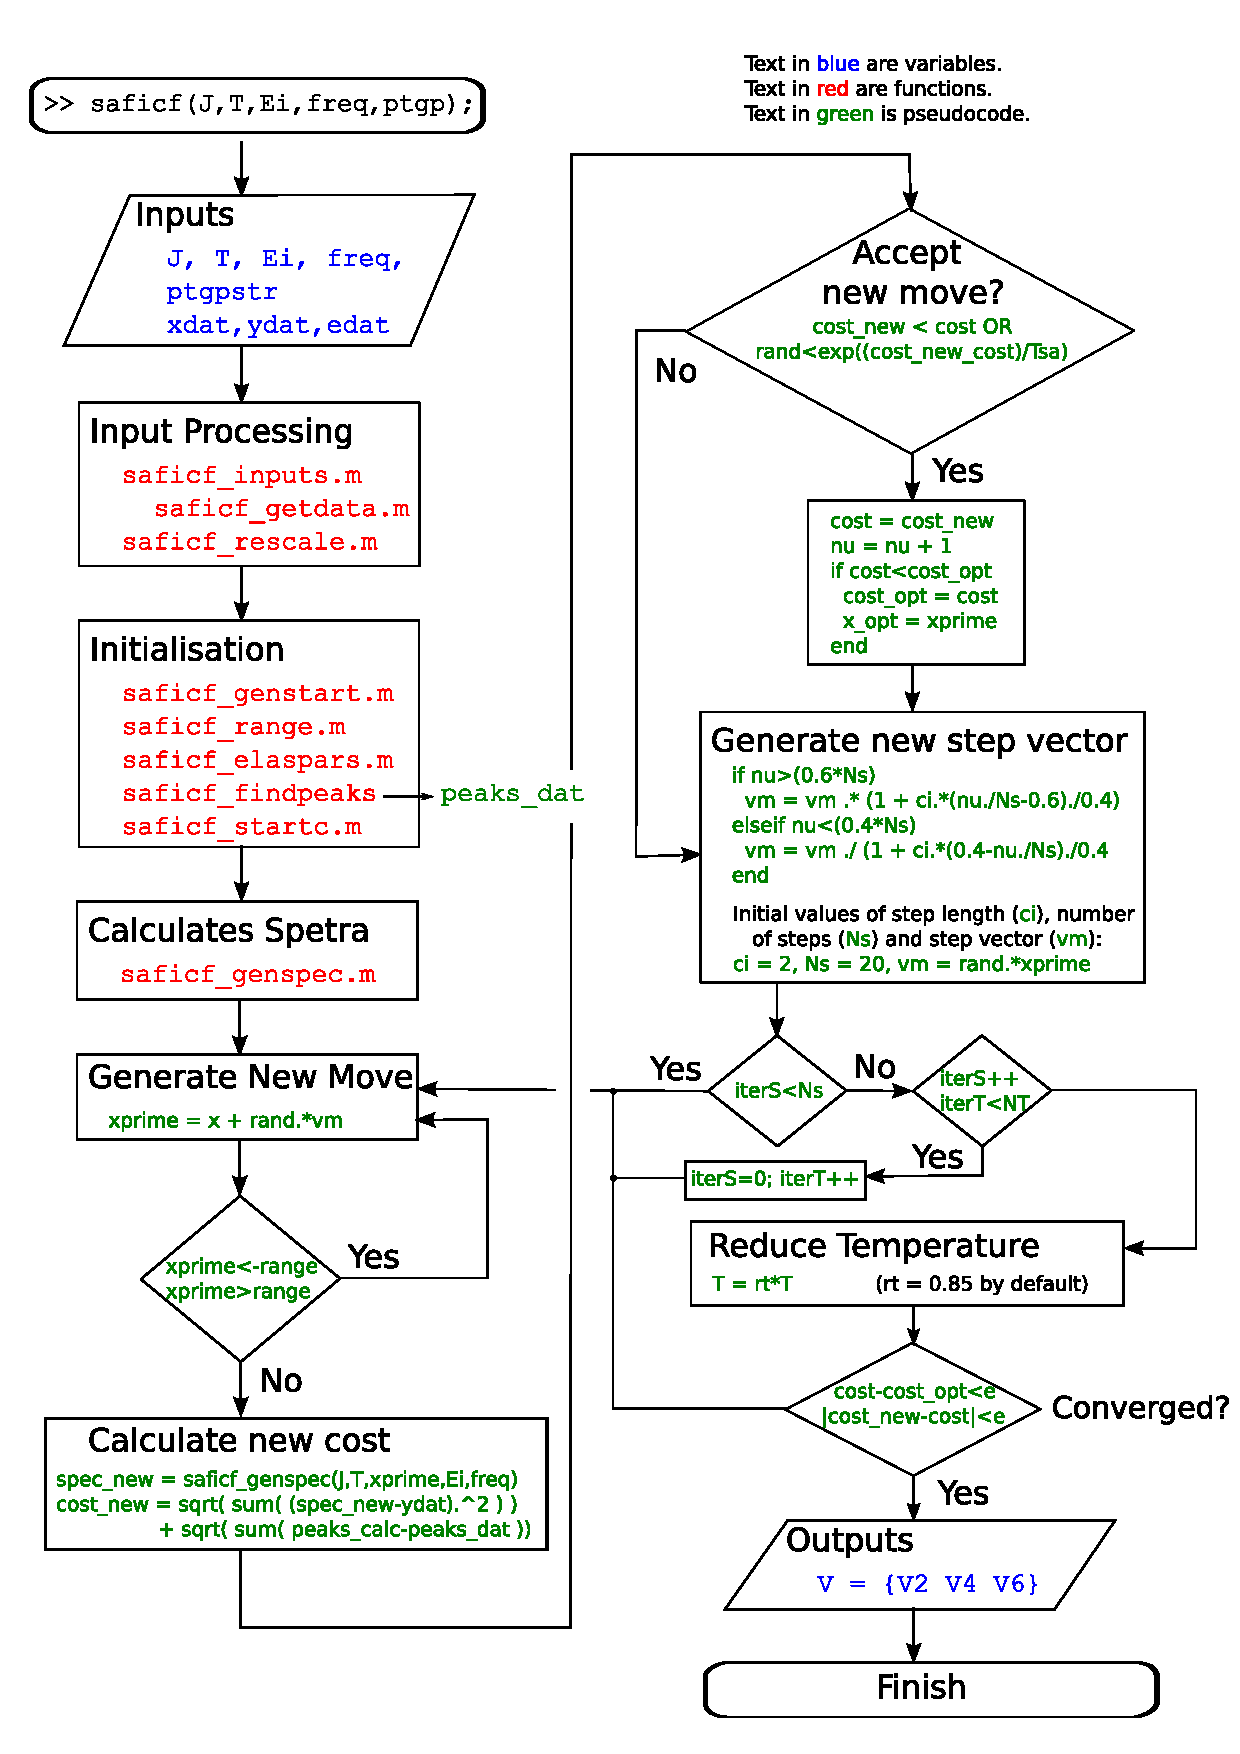
\includegraphics[width=0.9\textwidth, viewport=14 17 590 816]{figs/block.pdf}
    \caption{\emph{Block diagram of the SAFiCF program}.} \label{fg:block}
  \end{center}
\end{figure}

We simulate the inelastic neutron spectra (INS) of a magnetic ion in a crystal field using equations~\ref{eq:xsdipole} or~\ref{eq:Sqwdipole} as the user demands, or using simply the dipole transition probabilities given by the large curly brackets of either expression scaled by an arbitrary constant. These delta functions are then convoluted with Gaussian functions whose width are either set to a constant by the user, to be proportional to the energy transfer, or calculated from the chopper and instruments programmed in (at the moment for the spectrometers at ISIS). The area of the Gaussian are thus proportional to the dipole transition probabilities as in~\ref{eq:xsdipole} or~\ref{eq:Sqwdipole}. 

We also use the function \texttt{saficf\_findpeaks(xdat,ydat,edat)} to estimate the peak positions of the transitions observed in the spectra, and add to the cost function a root mean square difference term between the calculated and observed energies, in addition to the root mean square difference between the observed and simulated spectra:

\begin{equation}
\textrm{Cost} = \left( \sum_x \frac{( y(x)_\textrm{calc} - y(x)_\textrm{obs} )^2}{\textrm{error(x)}^2} \right)^{\sfrac{1}{2}} + \left( \sum_\textrm{transitions} (\Delta_{\textrm{calc}}-\Delta_{\textrm{obs}})^2 \right)^{\sfrac{1}{2}}
\end{equation}

\noindent This additional term helps to make the actual minima deeper, so that the algorithm will converge more accurately. 

Finally, \emph{SAFiCF} also handles multiple datasets taken at different temperatures, incident energy, and chopper frequencies\footnote{\emph{SAFiCF} is designed to fit time-of-flight neutron spectra}, and uses the function \texttt{saficf\_rescale(T,Ei,f,xdat,ydat,edat)} to rescale the data such that the elastic line is the same for each dataset. The function \texttt{saficf\_elaspars(xdat,ydat)} is used to fit the elastic line using a Levenberg-Marquardt algorithm.


%A numbered list:

%\begin{enumerate}

%\item Setup equipment
%\item Take measurements
%\item Analyse results

%\end{enumerate}

%A nonnumbered list:

%\begin{itemize}

%\item Voltmeter
%\item Oscilloscope

%\end{itemize}

%%% ----------------------------------------------------------------------
\section{Usage} \label{sec-use}

\emph{SAFiCF} has no graphical user interface (yet!), so it must be invoked on the Matlab command line. You must pass the total angular quantum number of the ground multiplet ($J$), the temperature, incident energy, chopper frequency and the point group symmetry of the magnetic ion to the \texttt{saficf} function. However, if you do not pass vectors (or cell arrays of vectors) for the $x$-data, $y$-data and error-data, the function will ask you to click on a graph window, and obtain the data from this graph window. Thus you may use for example, \emph{MSlice} to extract data into a 2D plot, and then get \emph{SAFiCF} to get this data, and attempt to fit it:

\begin{verbatim}
>> J = 4;       % e.g. Pr3+
>> T = 4;       % in Kelvin
>> Ei = 23;     % in meV
>> freq = 200;  % in Hz
>> ptgp = 'C6h' % e.g. Hexagonal
>> V = saficf(J,T,Ei,freq,ptgp);
\end{verbatim}

\noindent This assumes you have plotted the data on a graph using Matlab somewhere. Otherwise, you would invoke:

\begin{verbatim}
>> V = saficf(J,T,Ei,freq,ptgp,xdat,ydat,edat);
\end{verbatim}

\noindent where \texttt{xdat}, \texttt{ydat}, and \texttt{edat} are vectors or cell arrays of vectors. If you are fitting multiple datasets, then you would put the vectors of the data into a cell array, and make the variables \texttt{T}, \texttt{Ei}, and \texttt{freq} into vectors, in the order in which they correspond to the datasets. If you do not give \texttt{xdat}, etc., but \texttt{T}, etc., are vectors the function assumes that multiple datasets are being fitted, and the data should be obtained from graph windows. Please note that \emph{each dataset must be plotted on a separate graph window}. For example for three spectra taken at different temperatures, but with the same spectrometer configurations:

\begin{verbatim}
>> J = 4;
>> T = [4 77 300];
>> Ei = [23 23 23];
>> freq = [200 200 200];
>> ptgp = 'C6h'
>> V = saficf(J,T,Ei,freq,ptgp);
\end{verbatim}

\noindent Or alternatively:

\begin{verbatim}
>> xdat = {x1 x2 x3};
>> ydat = {y1 y2 y3};
>> edat = {e1 e2 e3};
>> V = saficf(J,T,Ei,freq,ptgp);
\end{verbatim}

There are also some functions which may be used independently of \texttt{saficf}. In particular, \texttt{cf\_hmltn} and \texttt{cflvls} may be used to calculate the crystal field Hamiltonian and the energy levels and dipole transition matrix elements for a specified set of CF parameters. For example, for Pr$^{3+}$ in a site of hexagonal symmetry, with $B_0^2 = 0.2$ meV,  $B_0^4 = 0.01$ meV,  $B_0^6 = 0.005$ meV, $B_6^6 = 0.003$ meV: 

\begin{verbatim}
>> J = 4;
>> B2 = [0 0 0.2 0 0 0];
>> B4 = [0 0 0 0 0.01 0 0 0 0];
>> B6 = [0 0 0 0 0 0 0.005 0 0 0 0 0 0.003]);
>> Hcf = cf_hmltn(J,B2,B4,B6);
>> T = 4;                                        % Temperature in Kelvin 
>> peaks = cflvls(Hcf,T)
\end{verbatim}

\noindent Note that the vectors for the CF parameters go from $B_{q=-k}^k$ to $B_{q=k}^k$. This invocation will also output a graph showing the levels and dipole allowed transitions with their associated matrix elements. Alternatively, you may output a two column vector of the inelastic cross-section in the dipole approximation, as in equation~\ref{eq:xsdipole}:

\begin{verbatim}
>> L = 5; S = 1;
>> peaks = cflvls(Hcf,J,[0 1],[1],[L S J])
\end{verbatim}

All the of functions are relatively well documented in the m-files, so you should not be afraid to read the source! In addition, you can use the inbuilt Matlab help commands to get information on how to use the functions:

\begin{verbatim}
>> help cf_hmltn
\end{verbatim}

Finally, there is also a function to use the Corana algorithm to fit an arbitrary function with the same syntax as \texttt{speclsqr}:

\begin{verbatim}
>> x = -5:0.1:5; 
>> y = fgauss(x,[-1.2 1 10])'+(rand(size(x))*2-1)*0.5; 
>> plot(x,y,'.');
>> p_in = [1 1 1];          % Guess parameters
>> dp_in = [0.1 0.1 0.1];   % Guess step in parameters
>> [p_lm,std_lm] = speclsqr(x,y,ones(size(x)),p_in,dp_in,@fgauss)
>> [p_sa,std_sa] = saficf_salsqr(x,y,ones(size(x)),p_in,dp_in,@fgauss)
\end{verbatim}

\noindent Please note that the Simulated Annealing routine whilst much less sensitive to the initial guess, \texttt{p\_in}, is also about 500-1000 times slower than the Levenberg-Marquardt algorithm in \texttt{speclsqr}.

%Figures:

%\begin{figure}
%  \begin{center}
%    \includegraphics[width=\textwidth]{tempfig.pdf}
%    \caption{\emph{Emphasis for caption title}. Caption.} \label{fg:test}
%  \end{center}
%\end{figure}

%A Table:

%\begin{figure}
%\begin{center}
%  \begin{tabular}{|l|r|r|r|}  % Format: l=left justified r=right justified c=centred
%   \hline % Horizontal line
%   & $10 \times 10$ & $14 \times 14$ & $20 \times 20 $ \\ \hline    % & denotes column breaks; \\ denotes row breaks
%   Least Slope & 0.83nm & 1.11nm & 1.52nm \\ 
%   Greatest Slope & 1.42nm & 1.33nm & 2.46nm \\
%   Average & $1.1 \pm 0.3$nm & $1.2 \pm 0.1$nm & $2.0 \pm 0.5$nm \\ \hline \hline 
%   & $30 \times 30$ & $40 \times 40$ & $50 \times 50$ \\ \hline
%   Least Slope & 5.63nm & 1.82nm & 5.3nm \\
%   Greatest Slope & 7.91nm & 3.02nm & 11.5nm \\
%   Average & $6 \pm 1$nm & $2.4 \pm 0.6$nm & $8 \pm 3$nm \\ \hline
%  \end{tabular}
%  \caption{\emph{Estimated widths of the wide barrier. The error estimates are obtained from comparing the greatest and least slopes.}} \label{tab:Width}
%\end{center}
%\end{figure}


%%% ----------------------------------------------------------------------

%\begin{thebibliography}{Bibliography}

% {\bf is boldfont}
%\bibitem{Sun05} L.F. Sun, S.N. Chin, E. Marx, K.S. Curtis, N.C. Greenham, C.J.B. Ford, \emph{Nanotechnology} {\bf 16} 631-634 (2005)
%\bibitem{Wothers} J.P. Clayden, N. Greeves, S. Warren, P.D. Wothers, \emph{Organic Chemistry}, Oxford University Press (2001)

%\bibliographystyle{plain}      % sorts authors alphabetically)
%\bibliographystyle{unsrt}      % does not sort authors
%\bibliographystyle{abbrv}      % abbreviates firstnames.
%\bibliographystyle{alpha}      % e.g. [SLE04]
%\bibliographystyle{siam}       % names in small-caps
%\bibliographystyle{apalike}    % e.g. [Skene et al., 2004]
%\bibliographystyle{e2subacm}
\bibliographystyle{apsrev}
%\bibliographystyle{elsart-num} % Elsevier style: Auts, \emph{Journ}, {\bf vol} (Year) pages
\bibliography{mdlrefs}          % Inserts bibliography files.

%\end{thebibliography}

%%% ----------------------------------------------------------------------

\newpage
\appendix
%\section*{Appendix}
%
%\section{Integration by parts} \label{ap-int}
%
%Use the equation:
%
%\[ \int_a^b u \frac{dv}{dx} dx = \left[ uv \right]_a^b - \int_a^b v \frac{du}{dx} \]


%%% ----------------------------------------------------------------------

%\section{Chain Rule} \label{ap-chainrule}
%
%Use the equation:
%
%\[ \frac{dy}{dx} = \frac{dy}{dt} \frac{dt}{dx} \]

%%% ----------------------------------------------------------------------


\end{document}
